%%%%%%%%%%%%%%%%%%%%%%%%%%%%%%%%%%%%%%%%%%%%%%%%%%%%%%%%%%%
% --------------------------------------------------------
% Tau
% LaTeX Template
% Version 2.4.4 (28/02/2025)
%
% Author: 
% Guillermo Jimenez (memo.notess1@gmail.com)
% 
% License:
% Creative Commons CC BY 4.0
% --------------------------------------------------------
%%%%%%%%%%%%%%%%%%%%%%%%%%%%%%%%%%%%%%%%%%%%%%%%%%%%%%%%%%%

\documentclass[12pt,a4paper,onecolumn,twoside]{tau-class/tau}
\usepackage[english]{babel}
\usepackage{parskip}
\usepackage{listings}

%% Spanish babel recomendation
% \usepackage[spanish,es-nodecimaldot,es-noindentfirst]{babel} 

%% Draft watermark
% \usepackage{draftwatermark}

%----------------------------------------------------------
% TITLE
%----------------------------------------------------------

\journalname{Architectural Design Prototype}
\title{Serverless Data Ingestion \& Event Driven Analytics Platform}

%----------------------------------------------------------
% AUTHORS, AFFILIATIONS AND PROFESSOR
%----------------------------------------------------------

\author{Yvonne Marneth and Jana Madison Burns-Balog}

%----------------------------------------------------------
% FOOTER INFORMATION
%----------------------------------------------------------

\institution{University of Upper Austria}
\footinfo{Project Report}
\theday{July 26, 2024}
\leadauthor{Marneth and Burns-Balog}
\course{Cloud Computing WS 2025/26}

%----------------------------------------------------------
% ABSTRACT AND KEYWORDS
%----------------------------------------------------------

\begin{abstract}    
    
\end{abstract}

%----------------------------------------------------------

\keywords{serverless, event-driven, data ingestion, cloud computing, project report}

%----------------------------------------------------------

\begin{document}

\maketitle
\thispagestyle{firststyle}
\tauabstract
% \tableofcontents
% \linenumbers 

%----------------------------------------------------------

\section{Original Project Vision}

\taustart{T}he original vision for this project was to create an event-driven analytics platform that makes use of serverless technologies in order to efficiently ingest, process and store data. The platform was intended to be scalable, flexible and resource-efficient by leveraging cloud services.

The basic pipeline consists of a client application that generates events and sends them to a serverless ingestion layer in the cloud. This ingestion layer is responsible for receiving the events and passing them to an event stream. From there, downstream processing functions can consume the events, perform analytics and store the results in a database.


\section{The client application}

The client application is a multiplatform mobile app developed using Kotlin Multiplatform Mobile (KMM). Its main purpose is to allow people who engage in Bouldering to log their climbing sessions and track the boulders they have climbed. The logging of climbing sessions thereby generates events that can be sent to the serverless ingestion layer. These events should be handled asynchronously in order to not block the user interface of the app and to sync data after periods of offline usage. Figure \ref{fig:app} shows the client application running on a mobile device.

\begin{figure}[h]
    \centering
    \includegraphics[width=0.5\columnwidth]{./figures/app.jpg}
    \caption{The client application on a mobile device.}
    \label{fig:app}
\end{figure}


\section{Choosing the cloud provider and services}

Choosing the right cloud provider and services for the prototype was a crucial step in the project. After evaluating various options, Google Cloud Platform (GCP) was selected, in order to experiment with Cloud Functions and Pub/Sub for the serverless ingestion layer and event streaming.

However, due to problems with our GCP account, we had to change plans and decided to use a private cloud based on OKD (OpenShift Kubernetes Distribution) for the implementation of the serverless ingestion layer and event streaming. This change would allow us to continue with the project while still exploring serverless and event-driven architectures, as well as gaining experience with Kubernetes-based solutions, which carry less vendor lock-in compared to managed cloud services.

However, this change also meant that we had to adapt our original vision and implementation plan to fit the capabilities and limitations of the private cloud environment. The architecture of the prototype is shown in Figure \ref{fig:architecture}.

\begin{figure}[h]
    \centering
    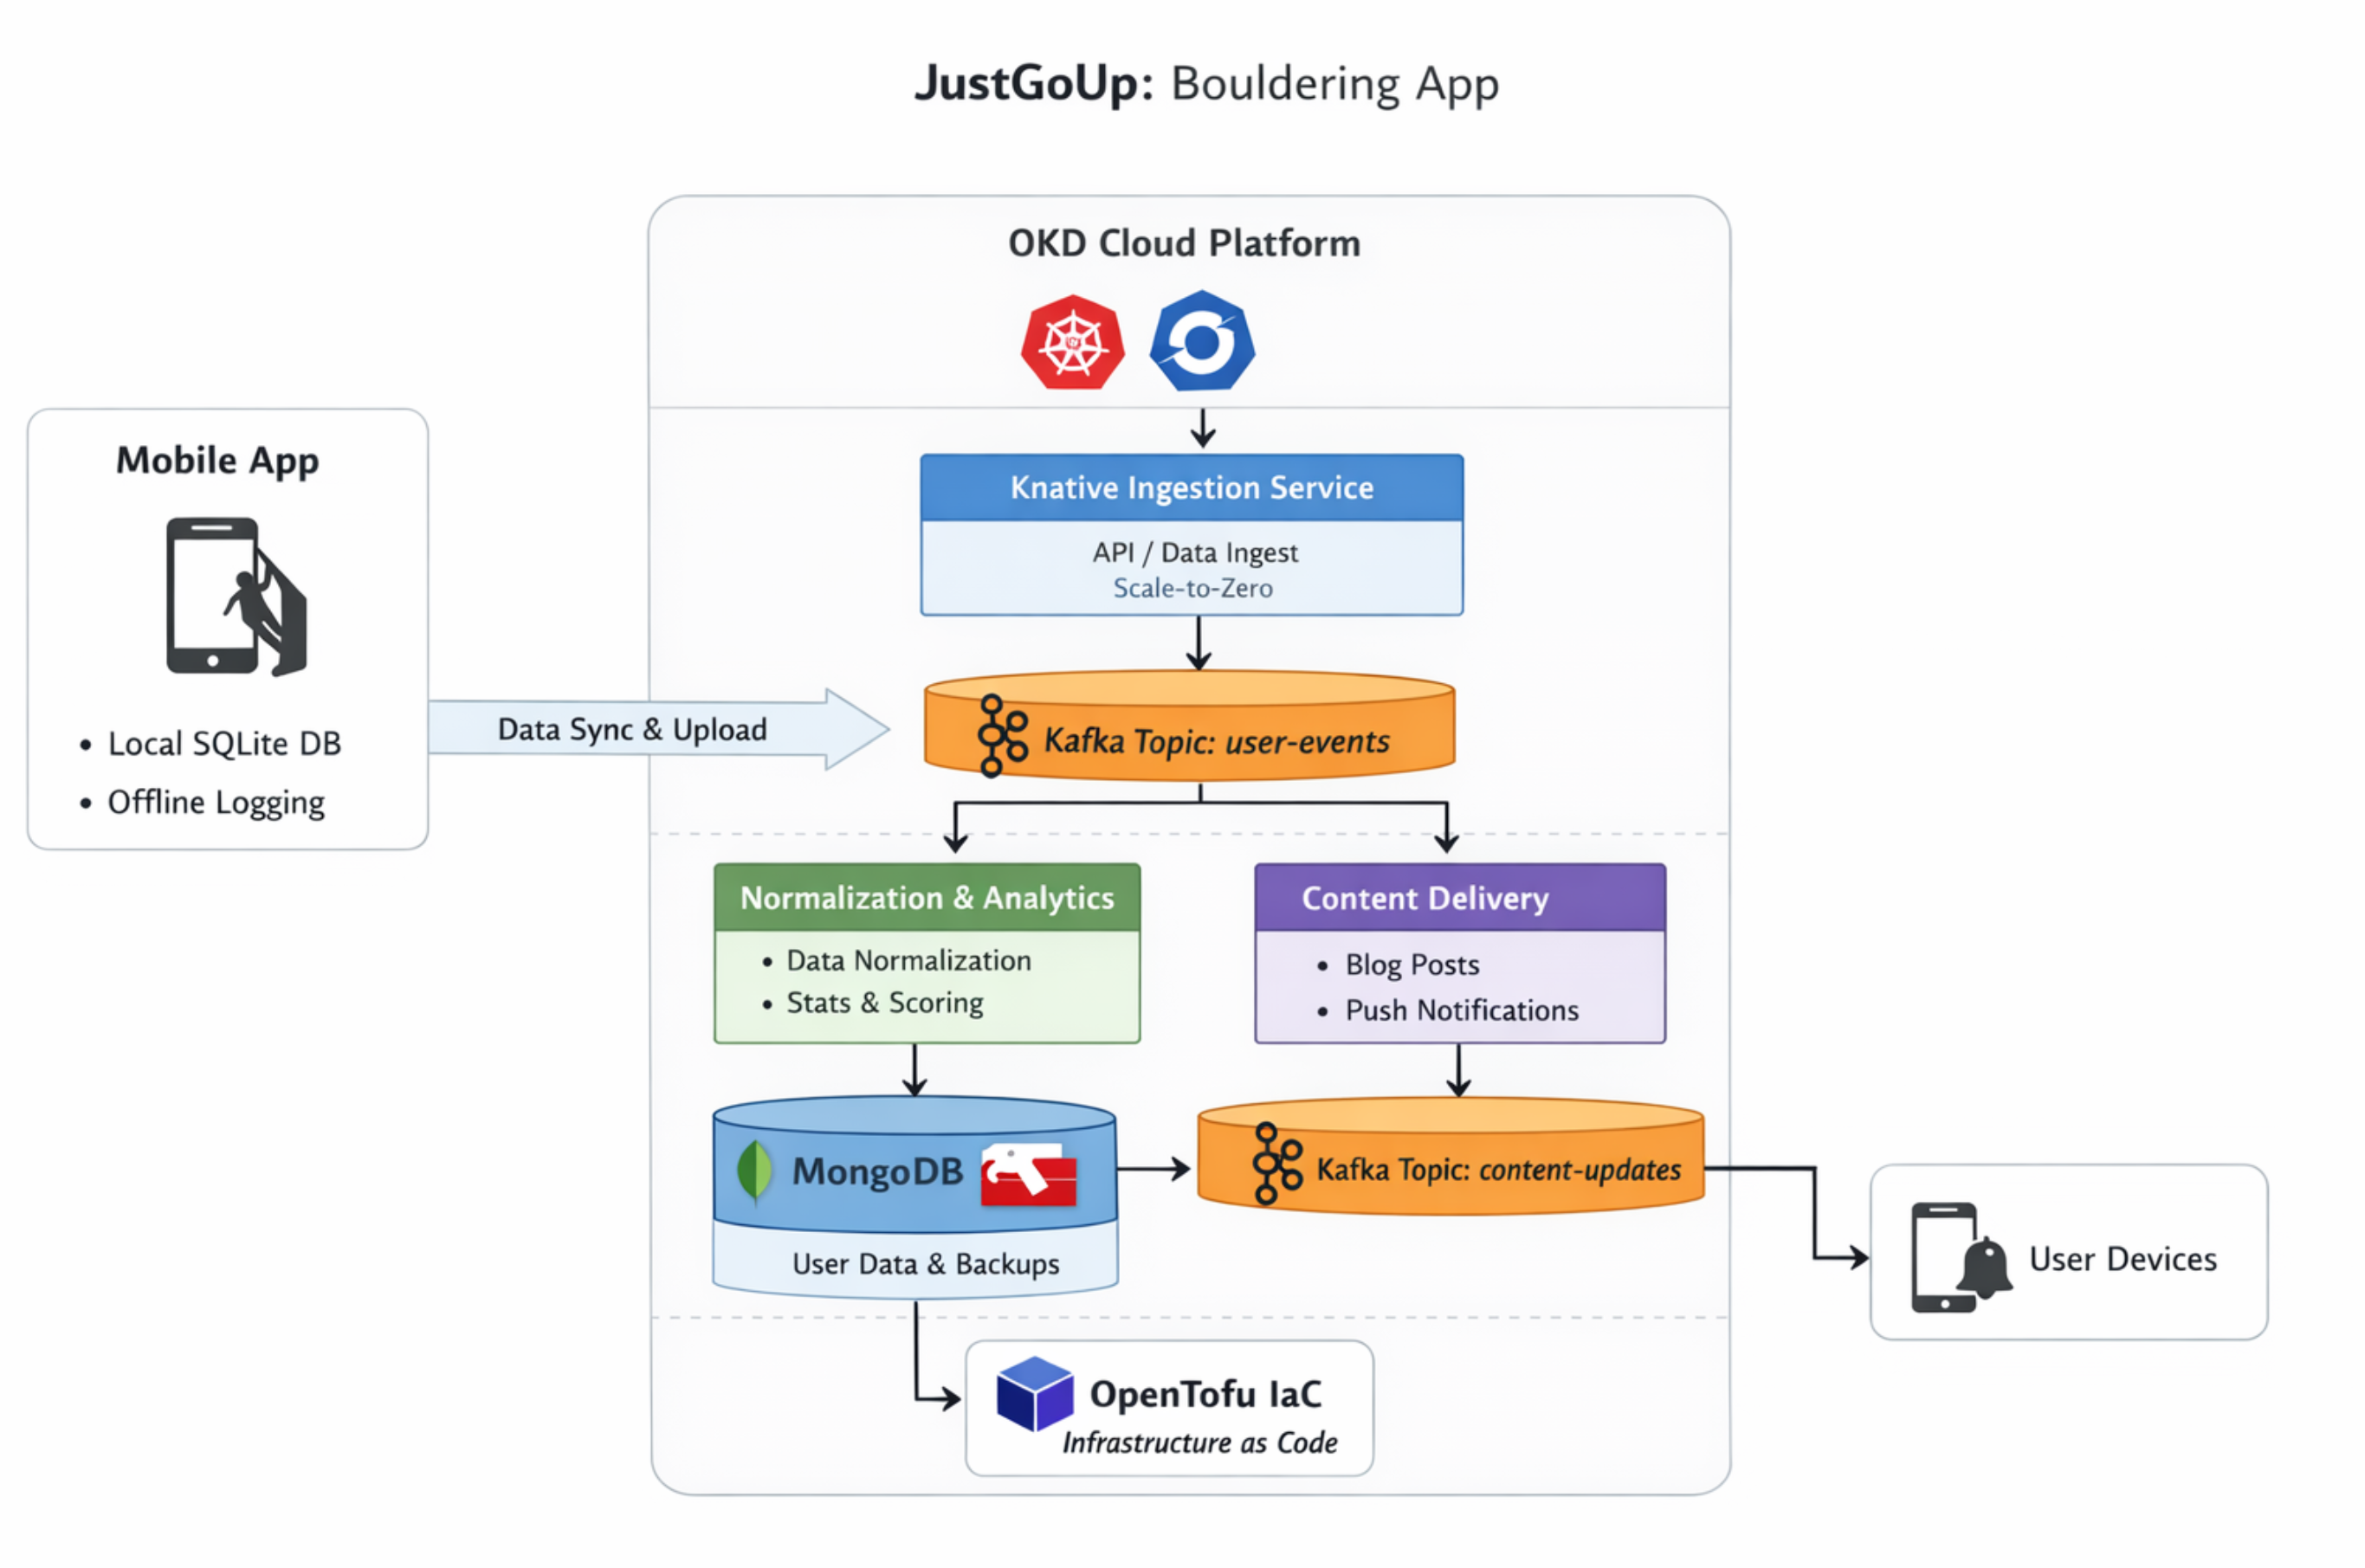
\includegraphics[width=0.75\columnwidth]{./figures/architecture.png}
    \caption{The architecture of the prototype.}
    \label{fig:architecture}
\end{figure}

\subsection{IaC provisioning - OpenTofu}

For the infrastructure provisioning of the private cloud environment, we decided to use OpenTofu, an Infrastructure as Code (IaC) tool, which is an open-source variant of Terraform. With OpenTofu, we were able to define and manage the infrastructure resources required for our serverless ingestion layer and event streaming in a declarative manner. The explicit goal was to follow a cloud-first approach, where the infrastructure is defined and managed through code, in order to ensure consistency and reproducibility.


\subsection{Serverless ingestion layer - Knative}

The serverless ingestion layer was implemented using Knative, a Kubernetes-based platform specifically designed for building and deploying serverless applications. Knative is also an open-source project, which aligns well with our choice of using a private cloud based on OKD. It provides an operator that should make it easy to install on the cluster and offers features such as automatic scaling, eventing and routing.

\subsection{Event streaming - Apache Kafka}

Kafka is a distributed event streaming platform that is widely used for building real-time data pipelines and streaming applications. It is a technology that we wanted to gain experience with, as it is a popular choice for event-driven architectures.

In hindsight, Kafka might have been an overengineered choice for our prototype, as our event streaming requirements were relatively simple and could have been fulfilled with simpler solutions. However, using Kafka provided us with valuable experience in working with a complex event streaming platform and understanding its capabilities and limitations.

\subsection{NoSQL data storage - MongoDB}

MongoDB was chosen as the data store for storing the climbing session data. The document-style storage model is perfect for the climbing session data, which can be represented as documents. MongoDB also offers scalability and schema flexibility, which are important for our use case.


\section{Implementation}

The implementation of the prototype was done in several steps, starting with the preparation of the cluster environment, followed by the development of the serverless ingestion layer and the event streaming components. The client application was developed in parallel.

\subsection{Preparing the cluster}

The first step was to set up the OKD cluster and install the necessary components. Knative was installed using the Knative operator, which simplified the installation process, but has to be done by the cluster administrator and therefore is not able to be provisioned automatically. Since using the Knative operator needs additional cluster roles, we had to wait for the cluster administrator. In order to start working on the implementation, we used a local Minikube cluster in the meantime. The operator can also be used to install Knative on Minikube.

The operator is installed by running the following command:

\begin{lstlisting}[language=bash, caption={Install Knative operator}]
# install the Knative operator    
kubectl apply -f https://github.com/knative/operator/releases/download/knative-v1.20.1/operator.yaml

# ensure the correct namespace is set
kubectl config set-context --current --namespace=knative-operator

# verify the installation
kubectl get deployment knative-operator
\end{lstlisting}

For the networking layer, we chose the Kourier Ingress, which is installed by creating a KnativeServing custom resource:

\begin{lstlisting}[caption={Install Knative operator}]
apiVersion: operator.knative.dev/v1beta1
kind: KnativeServing
metadata:
  name: knative-serving
  namespace: knative-serving
spec:
  ingress:
    kourier:
      enabled: true
  config:
    network:
      ingress-class: "kourier.ingress.networking.knative.dev"
\end{lstlisting}

Then, Knative Serving and Eventing can be installed using the operator:

\begin{lstlisting}[language=bash, caption={Install Knative operator}]
# install the Knative operator    
kubectl apply -f https://github.com/knative/operator/releases/download/knative-v1.20.1/operator.yaml

# ensure the correct namespace is set
kubectl config set-context --current --namespace=knative-operator

# verify the installation
kubectl get deployment knative-operator
\end{lstlisting}

\section{Tables and figures}

\subsection{Tables}

Table \ref{tab:table} shows an example table. The \verb|\tabletext{}| is used to add notes to tables easily.

\begin{table}[H]
    \centering
    \caption{Astronomical Object Data}
    \label{tab:table}
    \begin{tabular}{ll}
        \toprule
        \textbf{Object}  & \textbf{Distance (Light Years)} \\
        \midrule
        Alpha Centauri   & 4.37                            \\
        Betelgeuse       & 642.5                           \\
        Andromeda Galaxy & 2.537 million                   \\
        \bottomrule
    \end{tabular}

    \tabletext{Note: The table contains data of some famous celestial objects.}

\end{table}

\subsection{Figures}

Fig. \ref{fig:examplefloat} shows an example of two figures that covers the width of the page. It can be placed at the top or bottom of the page. The space between the figures can also be changed using the \verb|\hspace{Xpt}| command.

\begin{figure*}[t] % t for position at the top of the current page; b for position at the bottom; p for new page
    \centering
    \begin{subfigure}[b]{0.38\linewidth} % Fig (a)
        
\includegraphics[width=\linewidth]{Example2.pdf}
        \caption{Example left figure.}
        \label{fig:figa}
    \end{subfigure}
    \hspace{20pt}   % Space between the figures
    \begin{subfigure}[b]{0.375\linewidth} % Fig (b)
        
\includegraphics[width=\linewidth]{Example3.pdf}
        \caption{Example right figure.}
        \label{fig:figb}
    \end{subfigure}
    \caption{Example figure that covers the width of the page obtained from PGFPlots \cite{PFGPlots}.}
    \label{fig:examplefloat}
\end{figure*}

%----------------------------------------------------------

\printbibliography

%----------------------------------------------------------

\end{document}